\section{Introduction}
My topic I did my final Project about is related to my field of research, which is Speaker Recognition. In this field of research we try to find suitable model, which can predict if a given speech segment ( called utterance ) was spoken by a specific speaker. 
Generally speaking, we have usually a given set of $\mathbf{S} = \left\lbrace S_1 , S_2 , \ldots , S_n \right\rbrace$ speakers of which each produce an arbitrary mount ($q$) speech segments, which we have as our basic data. We try to find the most probable hypothesis that a newly, unheard-of of speech segment, belongs to any of the given speaker set $\mathbf{S}$.
To accomplish this task we assume having two different models, which try to identify a newly heard utterance $u$:
\begin{align*}
H_0 &= u \text{ is spoken by } S\\
H_1 &= u \text{ is spoken not by } S\\
\end{align*}
$H_0,H_1$ represent here the models for the correct speakers ($H_0$) and the wrong ones (or impostors $H_1$).
So we need only to define a threshold $t$ which indicates if the utterance $u$ is either belonging to $H_0$ or $H_1$. Then we can rewrite:
\begin{gather*}
\frac{P(u|H_0)}{P(u|H_1)} = \begin{cases}
\leq t, \text{ accept } H_0\\
> t , \text{ accept } H_1
\end{cases}
\end{gather*}
The important part is to find robust and versatile models for $H_0$ and $H_1$ respectively.

In the field of speech recognition, the input consists of raw waveforms, which will be transformed into so called features. Features are basically an extracted vectorized form of the original signal. Their purpose is to reduce the dimensionality complexity for further processing, since the overall amount of raw data is simply too arduous to handle.

\section{Motivation}

The motivation for this Project comes from the real world application of feature extraction and speech Processing. Nowadays the amount of data for training any kinds of models is extremely large ( hundreds of Gigabytes), so that one needs to extract only the meaningful information out of the data. This process is called feature extraction and results in a vectorized representation of the data. Using these feature vectors, we can train a model, which goal it is to classify a certain behaviour. This final model can then be post-processed by LDA to increase the distances between the classes. 
LDA is a general post-processing tool in speaker recognition. In this Report we show how LDA can also be used by using the power iteration instead of the more general QR-Decomposition.

\section{Linear Discriminative Analysis}
%Blabla basisc about LDA

For speaker recognition we use LDA to improve our improve our scores. It is widely used after the computation of the models $H_0$ and $H_1$ to project the resulting high-dimensional vectors into a lower dimensional space, where the separation between the involving classes is maximized.

To achieve a dimensionality reduction, we use

Assume having $c$ classes in an arbitrary space. We calculate the proportion in between the between-class covariance and the within-class covariance, having the current feature vector $\mathbf{x}_i$:
\begin{align*}
\mathcal{L} ( \mathbf{w} ) &= - \frac{\mathbf{w}^T \Sigma_{\text{between}} \mathbf{w}}{\mathbf{w}^T \Sigma_{\text{within}} \mathbf{w}} \\
\Sigma_{\text{within}} &= \sum_i^c \Sigma_i \\
\Sigma_i &= \sum_i^c \left( \mathbf{x} - \boldsymbol{\mu}_i  \right) \left( \mathbf{x} - \boldsymbol{\mu}_i \right)^T\\
\Sigma_{\text{between}} &= N_i \sum_i^c \left( \boldsymbol{\mu}_i - \boldsymbol{\mu} \right) \left( \boldsymbol{\mu}_i - \boldsymbol{\mu} \right)^T
\end{align*}
where $\boldsymbol{\mu}_i$ is the mean of the current class, $\boldsymbol{\mu}$ the overall mean and $N_i$ is the sample mean of the $i$-th class.

As soon as the covariances are calculated, we need to focus on how to compute the weight vectors $\mathbf{w}$. We solve this generalized eigenvalue problem by calculating the eigenvalues of:
\begin{align*}
\sigma\left( \Sigma_{\text{within}}^{-1}\Sigma_{\text{between}} \right) = \left\lbrace \lambda_1 , \lambda_2 , \ldots,\lambda_n \right\rbrace
\end{align*}
With these eigenvalues we compute the corresponding eigenvectors. 
The clue of the whole algorithm is then to use the most important $m, m< n$ eigenvalues, to construct the overall weight matrix $\boldsymbol{W}$, which then projects the input features into the new $m$ dimensional feature space.
\begin{align*}
\mathbf{y} = \mathbf{W}^T \mathbf{x}
\end{align*}

A large eigenvalue means that the corresponding eigenvector has also large values, which means that this eigenvector encompass most of the variance of the given class. This means we can simply sort the eigenvalues in descending order and pick the largest $m$ eigenvalues out. Doing so allows us to reduce the dimensionality of the given data, by removing the less important parts.
\begin{figure}[h]
\centering
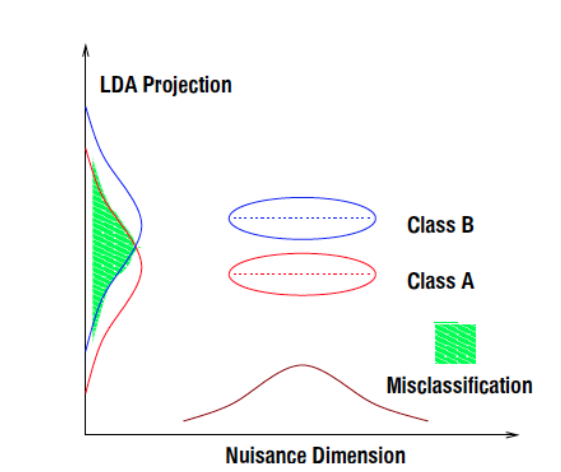
\includegraphics[scale=0.4]{LDA.png}
\caption{Using LDA to increase inner class distance in case of constant covariance }
\end{figure}

Here we want to point out that there exist many different algorithms for computing the eigenvalues, whereas we have focused in this Report in the Power iteration. 

\subsection{Power Iteration}
In mathematics, the power iteration is an eigenvalue algorithm: given a matrix $\mathbf{A}$, the algorithm will produce a number $\lambda$ (the eigenvalue) and a nonzero vector $\mathbf{v}$ (the eigenvector), such that $\mathbf{Av} = \mathbf{\lambda v}$.

The power iteration algorithm starts with a vector $\mathbf{b}_0$, which may be an approximation to the dominant eigenvector or a random vector. The method is described by the iteration $ b_{k+1} = \frac{Ab_k}{\|Ab_k\|}$.
So, at every iteration, the vector $\mathbf{b}_k$ is multiplied by the matrix $\mathbf{A}$ and normalized.

Under the assumptions:
\begin{itemize}
\item $\mathbf{A}$ has an eigenvalue that is strictly greater in magnitude than its other eigenvalues
\item The starting vector $\mathbf{b_{0}}$ has a nonzero component in the direction of an eigenvector associated with the dominant eigenvalue.
then:
\item $\mathbf{A}$ subsequence of $\left( b_{k} \right)$ converges to an eigenvector associated with the dominant eigenvalue
\end{itemize}

Note that the sequence $\left( b_{k} \right)$ does not necessarily converge. It can be shown that:
$b_{k} = e^{i \phi_{k}} v_{1} + r_{k}$ where: $v_{1}$ is an eigenvector associated with the dominant eigenvalue, and  $\| r_{k} \| \rightarrow 0$. The presence of the term $e^{i \phi_{k}}$ implies that $\left( b_{k} \right)$  does not converge unless $e^{i \phi_{k}} = 1$ Under the two assumptions listed above, the sequence $\left( \mu_{k} \right)$ defined by: $\mu_{k} = \frac{b_{k}^{*}Ab_{k}}{b_{k}^{*}b_{k}}$ converges to the dominant eigenvalue.

It needs to said that $b_k$ converges to a multiple of the eigenvector $\mathbf{v}_1$, at rate $ \left| \frac{\lambda_2}{\lambda_1} \right| $, where $\lambda_2$ is the second dominant eigenvalue. Thus, the method converges slowly if there is an eigenvalue close in magnitude to the dominant eigenvalue.

\section{Experiments}

Generally speaking, when using real speech data, the dimensionality of the feature vectors it too large to efficiently display in any plot.
Therefore the following experiments are artificial and only show how LDA works. We sampled $n$ Gaussians with feature size of $2$, which will be reduced to $1$ dimensional features using LDA.

Moreover we have overall $1000$ samples for each Gaussian, meaning that we have overall $3000$ data points, characterized by a Gaussian distribution. 
Real data in speaker verification consists of $39$ dimensional vectors. The amount of data is generally measured in hours, whereas we can expect that per 100 MB data, we achieve about 1 hour of raw wave speech.


We used Python2.7 with the help of numpy to do the calculations. Generating the artificial data, we can simply use:


\begin{minted}[mathescape,
               numbersep=5pt,
               linenos,
               frame=lines,
               framesep=2mm]{python}
import numpy as np

means = np.random.randint(-10,10,size=(dims))
variances = np.random.sample(size=(dims,dims))
#We sample 3 classes with 1000 datapoints
datapoints = np.random.multivariate_normal(means,variances,size=(3,1000)).T
\end{minted}

In the chosen programming language, the power iteration is implemented as follows:

\begin{minted}[mathescape,
               numbersep=5pt,
               linenos,
               frame=lines,
               framesep=2mm]{python}
               
def powerIteration(A):
    b = [random() for i in range(len(A))]
    tmp = [0] * len(A)

    for iteration in range(1000):

        for i in range(0, len(A)):
            tmp[i] = 0
            for j in range(0, len(A)):
                tmp[i] += A[i][j] * b[j]

        normSq = 0
        for k in range(0, len(A)):
            normSq += tmp[k] * tmp[k]
        norm = sqrt(normSq)

        for i in range(len(A)):
            b[i] = tmp[i] / norm

    return b
\end{minted}

The LDA process was implemented in the following fashion, given the power iteration:
\begin{minted}[mathescape,
               numbersep=5pt,
               linenos,
               frame=lines,
               framesep=2mm]{python}
def lda(datapoints,tarDim = 2):
    '''
    datapoints is the given data, with shape [classsize samplesize featuredim]
    tarDim is the amount of eigenvalues which will be kept, meaning the dimension, which will be 
    transferred to
    '''
    cl,samplesize,featuresize = datapoints.shape
    mean_vectors=[]
    for i in range(cl):
        mean_vectors.append(np.mean(datapoints[i],axis=0))
#         print('Mean Vector class %s: %s\samplesize' % (i,mean_vectors[i]))
#     Calcuate Within Scatter matrix:
    mean_vectors = np.array(mean_vectors)
    s_w = np.zeros((featuresize,featuresize))
    
    for i in range(cl):
        curmat = datapoints[i]
        for row in curmat:
#             Get the current row, transform to col just for dot product purpose
            col = row.reshape(featuresize,1)
            meancol = mean_vectors[i].reshape(featuresize,1)
            s_w += (col-meancol).dot((col-meancol).T)
#         print ('Within class covaricance Scatter : ',s_w[i])
    overall_mean = np.mean(mean_vectors, axis=0)
    s_b = np.zeros((featuresize,featuresize))
    for i in range(cl):
        samp_size = len(datapoints[i])
        mean_row = mean_vectors[i].reshape(featuresize,1)
        s_b += samp_size*(mean_row - overall_mean).dot((mean_row-overall_mean).T)
    
    eig_vals,eig_vecs = powerIteration((s_w).dot(s_b))
    eig_pairs = [(np.abs(eig_vals[i]), eig_vecs[:,i]) for i in range(len(eig_vals))]
    eig_pairs = sorted(eig_pairs,key=lambda k: k[0] ,reverse=True)
    w= np.hstack(eig_pairs[i][1].reshape(featuresize,1) for i in range(tarDim))
    datapoints = datapoints.reshape(cl*samplesize,featuresize)
    x_lda = w.T.dot(datapoints.T)
    x_lda = x_lda.reshape(cl,samplesize)
    
    log.debug("XLDA Dim {0}".format(x_lda.shape))
    return x_lda
\end{minted}



\section{Results}

As we can see, the newly projected space maximizes the distance in between the classes effectively. In this reduced space, a classification can be easier performed, leading to an overall better classification performance. Moreover the computational cost is minor, so that LDA should be used whenever possible.

\begin{figure}
\centering
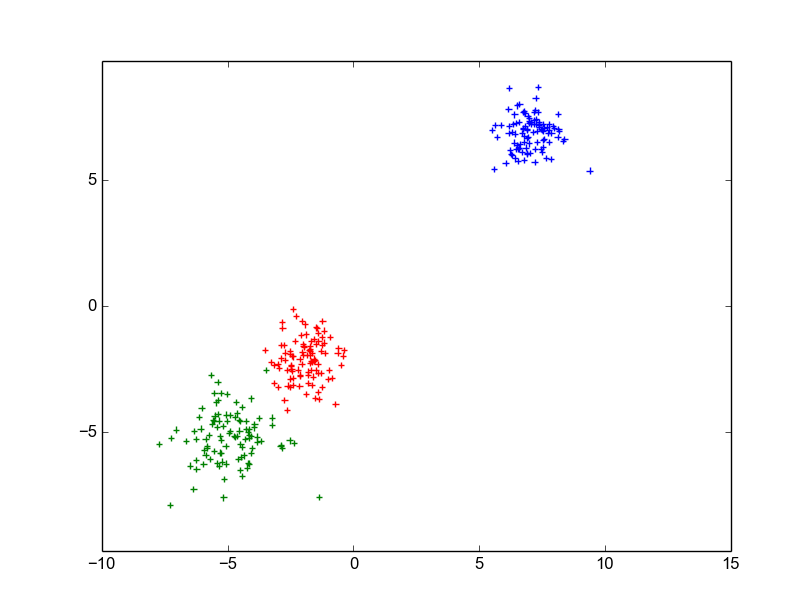
\includegraphics[scale=0.4]{3class_gauss.png}
\caption{3 Class Gaussian Randomly drawn out of 1000 samples}

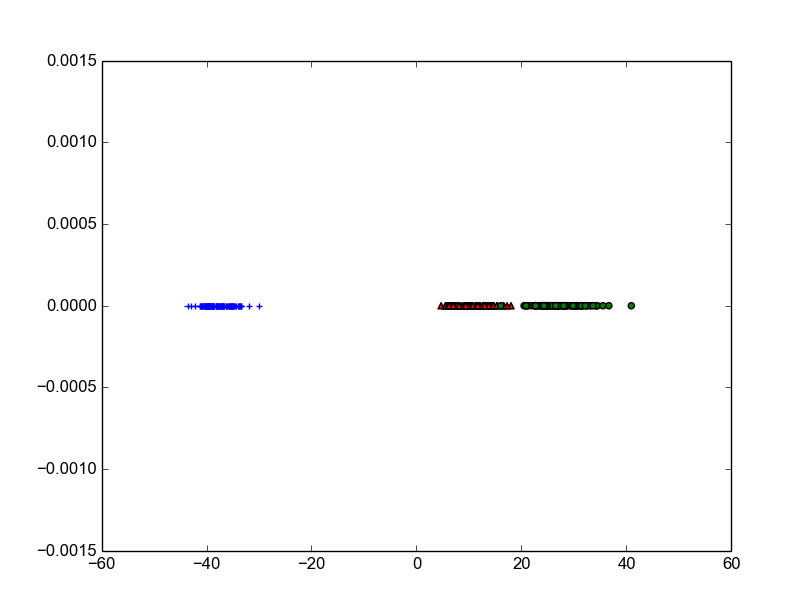
\includegraphics[scale=0.4]{3class_gauss_proj.png}
\centering
\caption{Projection of 3 Class Gaussian into 1 dimensional space}
\end{figure}

A subset of the generated used numbers can be seen here:
\begin{minted}[mathescape,
               numbersep=5pt,
               frame=lines,
               framesep=2mm]{python}
#Source data:
[[ 7.90729539  8.17202412  7.47519462]
 [ 9.55144994  8.37470264  7.88132993]
 [ 8.80252236  7.41339669  6.96571076]
 [ 9.27757307  6.47732587  9.34183583]]
# LDA Projection:
 [ 12.81458458  13.66795127  12.18943162  13.03469284]
\end{minted}

In the figures shown, we can see how LDA projects the initial 2 dimensional space into a single dimension. The power iteration helped us to find this single dimension quickly, since it converged within the first 30 iterations.
